% ==============================================================
\section{付録}\label{sec:supplement}
% ==============================================================

\subsection{EX7: パラメータ感度}
\label{sec:supp_ex7}

EX1の語彙内データ（$\beta = 0.3$ 固定）を用いて，
主要パラメータに対する頑健性を評価する（各3 seeds）．

\begin{figure}[h]
\centering
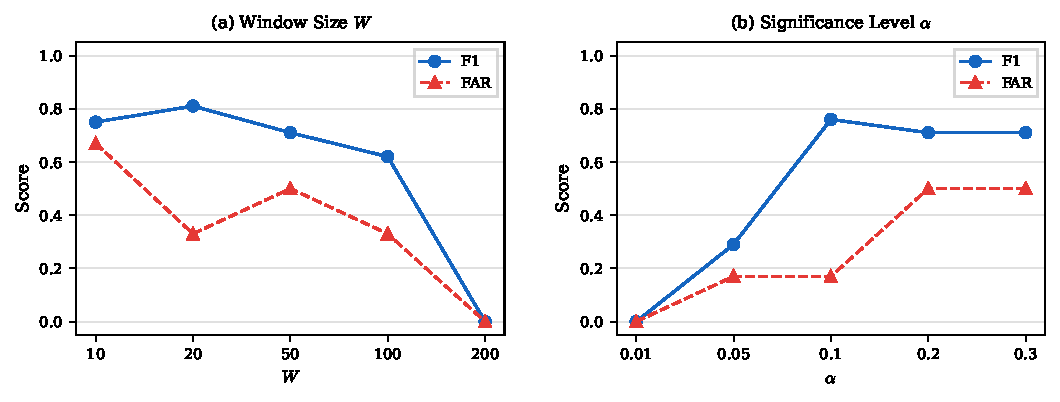
\includegraphics[width=\linewidth]{fig/sensitivity.pdf}
\caption{EX7: パラメータ感度（3 seeds平均）．(a) ウィンドウサイズ $W$: $W = 20$ で最高 F1 = 0.81，$W = 200$ では平滑化により検出不能．(b) 有意水準 $\alpha$: $\alpha = 0.10$ で最良のF1/FARバランス（F1 = 0.76, FAR = 0.17），$\alpha \leq 0.05$ ではBH補正により真の帰属も棄却されF1が急落．}
\label{fig:sensitivity}
\end{figure}

\subsubsection{置換回数 $B$}

\begin{table}[h]
\caption{EX7: 置換回数感度（3 seeds平均）}
\label{tab:ex7_perm}
\centering
\begin{tabular}{ccc}
\toprule
$B$ & F1 & 実行時間 (ms) \\
\midrule
50    & 0.71 & 913 \\
100   & 0.71 & 914 \\
500   & 0.71 & 941 \\
1{,}000 & 0.71 & 969 \\
5{,}000 & 0.71 & 1{,}201 \\
\bottomrule
\end{tabular}
\end{table}

全 $B$ 値で F1 = 0.71 と完全に安定しており，
置換回数に対して頑健である．
$p$ 値の分解能（$1/(B+1)$）を確保するため $B = 5{,}000$ を
デフォルトとする．

\subsubsection{変化点検出法}

閾値交差法とCUSUMを比較した結果，
語彙内ブースト条件では両手法ともF1 = 0.71で同等の精度を示した．

\subsection{EX8: スケーラビリティ}
\label{sec:supp_ex8}

\begin{figure}[h]
\centering
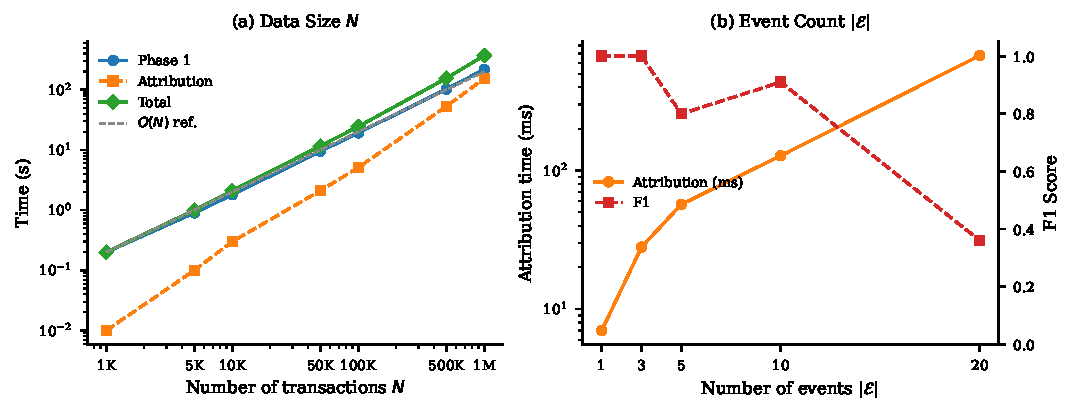
\includegraphics[width=\linewidth]{fig/scalability.pdf}
\caption{EX8: スケーラビリティ．(a) データサイズ $N$: Phase 1 と Attribution の両方が$N$に対して線形にスケールする．100万トランザクションで約6.2分．(b) イベント数 $|\mathcal{E}|$: 帰属時間は$|\mathcal{E}|$に対して線形．$|\mathcal{E}| \leq 10$ でF1 $\geq 0.80$，$|\mathcal{E}| = 20$ ではイベント密集により弁別力が低下しF1 = 0.36．}
\label{fig:scalability}
\end{figure}
